\documentclass{article}

\usepackage{geometry}
\usepackage{makecell}
\usepackage{array}
\usepackage{multicol}
\usepackage{setspace}
\usepackage{changepage}
\usepackage{booktabs}
\usepackage[explicit]{titlesec}
\usepackage{hyperref}
\usepackage{graphicx}
\usepackage{cprotect}
\usepackage{float}
\usepackage{wrapfig}
\newcolumntype{?}{!{\vrule width 1pt}}
\newcommand{\paragraphlb}[1]{\paragraph{#1}\mbox{}\\}
\renewcommand{\contentsname}{Inhaltsverzeichnis:}
\renewcommand\theadalign{tl}
\setstretch{1.10}
\setlength{\parindent}{0pt}

\titleformat{\section}
  {\normalfont\Large\bfseries}{\thesection}{1em}{\hyperlink{sec-\thesection}{#1}
\addtocontents{toc}{\protect\hypertarget{sec-\thesection}{}}}
\titleformat{name=\section,numberless}
  {\normalfont\Large\bfseries}{}{0pt}{#1}

\titleformat{\subsection}
  {\normalfont\large\bfseries}{\thesubsection}{1em}{\hyperlink{subsec-\thesubsection}{#1}
\addtocontents{toc}{\protect\hypertarget{subsec-\thesubsection}{}}}
\titleformat{name=\subsection,numberless}
  {\normalfont\large\bfseries}{\thesubsection}{0pt}{#1}

\hypersetup{
    colorlinks,
    citecolor=black,
    filecolor=black,
    linkcolor=black,
    urlcolor=black
}

\geometry{top=12mm, left=1cm, right=2cm}
\title{\vspace{-1cm}Webtechnologien und Usability}
\author{Andreas Hofer}

\begin{document}
	\maketitle
	\tableofcontents
	\newpage
	\section{Einführung}
	Das Internet ist ein System verbundener Netzwerk, welche mit Protokollen interagieren. Diesen Protokollen liegt das Packet Switching zugrunde. Das Internet ist jedoch nicht das World Wide Web (WWW), welches nur eine Anwendung ist die auf einem Hypermediasystem basiert. Das WWW enthält Resourcen und Links, welche diese miteinander verbinden und baut auf 3 Grundkonzepten auf:
	\begin{itemize}
		\item{Hypertext Transfer Protocol (HTTP)}
		\begin{itemize}
			\item{Erlaubt Zugriff auf Ressourcen eines Webservers. Das geschieht mittels Anfragen und Antworten (Requests und Responses)}
		\end{itemize}
		\item{Uniform Resource Identifier (URI)}
		\begin{itemize}
			\item{Erlaubt die eindeutige Identifizierung von Resourcen (Web Adressen)}
			\item{In der Vergangenheit gab es mehrere verschiedene Protokolle, welche durch das URI ersetzt wurden.}
		\end{itemize}
		\item{Hypertext Markup Language (HTML)}
		\begin{itemize}
			\item{Textbasierte Markupsprache (Auszeichnungssprache)}
			\item{Markup erlaubt die Gliederung und Formatierung von Daten, welche danach von einem Webbrowser interpretiert wird.}
			\item{Hyperlinks erlauben Verweise zwischen HTML Dokumenten}
		\end{itemize}
	\end{itemize}
	\subsection{Uniform Resource Identifier (URI)}
	URI erlaubt nicht nur die Verwendung von HTTP Adressen, sondern auch anderen wie mailto (Zum Versenden von E-Mails) oder FTP. \\
	URIs haben stets eine spezielle Formattierung: \verb|<scheme>:[authority]<path>[?<query>][#<fragment>]|. \\
	Das scheme identifiziert den Typ der Ressource wie zum Beispiel HTTP oder mailto. \\
	Die authority gibt die Domäne an, welche angesprochen wird. Eine solche Domäne kann eine Portnummer sein. (Siehe 1/NET1/5.7 [TODO Netzwerk]) \\
	Der path dient zur Identifizierung einer Ressource und kann aus mehreren Teilen bestehen, welche durch  Schrägstriche "/" getrennt sind.\\
	Die query ist Zusatzinformation, welche an den Server übergeben werden soll und folgt immer einem Fragezeichen "?". Mehrere queries können durch das Ampersand getrennt werden "\&". \\
	Das fragment gibt an, welche Teile auf der angefragten Seite gesucht werden.
	\subsubsection{URL und URN}
	Der Uniform Resource Locator (URL) und Uniform Resource Name (URN) sind zwei Teile der URI. Obwohl beide unter URI Verwendung finden, wird URL oft als synonym zu URI gesehen, da eine URN nur über die URL angesprochen werden kann. Die URN beschreibt den Namen der Resource und wird in dem Schema \texttt{urn:1234-5678-9012} angegeben. Diese finden unter anderem für Bücher Verwendung um die ISBN (International Standard Book Number) zu beschreiben.
	\section{Hypertext Markup Language (HTML)}
	HTML ist die grundlegende Resource, welche alle Websites verwenden. HTML gibt die Struktur, sowie die Formatierung für eine Seite an. Ein HTML Dokument kann zusätzlich zu der Struktur auch Javascript (JS) zur dynamischen Veränderung der Website, sowie Cascading Style Sheets (CSS) zum Styling der Element enthalten. \\
	HTML ist momentan in der fünften Version mit HTML 5. Der Name HTML besteht aus zwei Teilen: Hypertext sowie Markup Language. \\
	Hypertext ist ein Netzwerk an Dokumenten, welche wie ein Netz untereinander verbunden sind. Eine Markup Language ist eine Formatierungsstrategie, in welcher spezifische Teile mit Kennern ausgezeichnet werden können, welche danach in einer bestimmten Weise interpretiert werden. \\
	Eine Website besteht in der Regel aus mehr als einem einzelnen HTML Dokument sondern einer ganzen Sammlung welche jeweils untereinander verlinken und so die Erscheinung einer dynamischen Website geben können. Der Einstiegspunkt einer Website wird \texttt{index.html} genannt und dient als Anfangspunkt für die Navigation. \\
	\subsection{Elemente}
	Ein HTML Dokument besteht stets aus Elementen, welche die Struktur des Dokuments angeben. In diesen Elementen befinden sind eine oder mehrere HTML Attribute, welche jeweils ausgezeichnet werden. \\
	HTML Elemente besitzen in der Regel stets einen Start- und einen End-Tag, welche normalerweise mit größer- und kleiner gleich Zeichen ausgzeichnet werden: \texttt{<p> This is a paragraph </p>}. Ein End-Tag wird zusätzlich mit einem Slash "/" gekennzeichnet.
	\subsubsection{inline und block}
	Ein Element innerhalb eines HTML Dokuments ist stets im \texttt{inline} oder \texttt{block} Modus. Block bedeutet, dass es stets in seiner eigenen Zeile geführt wird. Also wird ein Block Element selbst ohne einem line break \texttt{<br>} in die nächste Zeile gesetzt und das nächste Element wird wiederum in der Zeile darunter. Ein inline Element hingegen kann direkt zwischen Text eingefügt werden und verbraucht genau so viel Platz wie das Element benötigt.
	\begin{figure}[H]
	\centering
	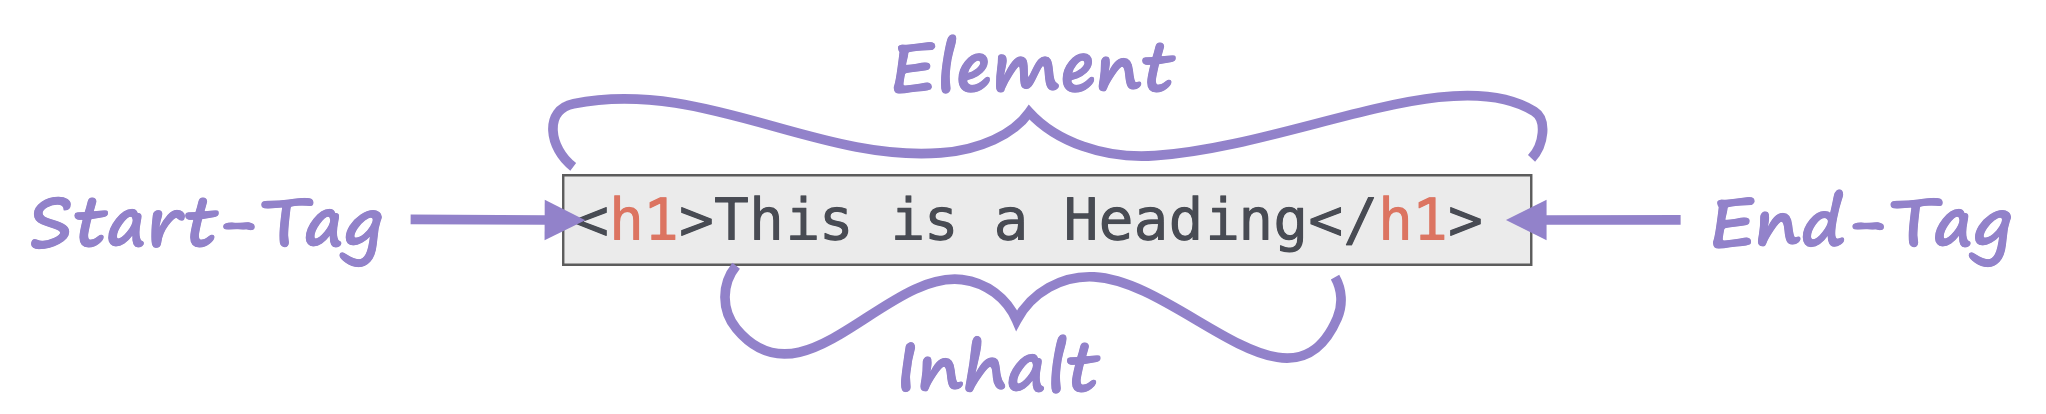
\includegraphics[scale=0.4]{Bilder/tag.png}
	\caption{Ein HTML Element sowie Start und End Tag}
	\end{figure}
	Zusätzlich gibt es auch leere Elemente, welche keinen End tag benötigen. \texttt{<br>} welches einen Line Break signalisiert, muss nicht wieder geschlossen werden. Zu beachten ist, dass Elemente sich nicht überlappen dürfen. Wenn man in einen Paragraphen begonnen hat, kann man nicht dazwischen ein anderes Element öffnen, jedoch nicht wieder schließen. \\
	HTML ist nicht case sensitive, jedoch ist es gute Form Tags stets mit Kleinbuchstaben zu schreiben. \texttt{Statt <P> eher <p>}\\
	Ein HTML Dokument beinhaltet seinen gesamten Inhalt innerhalb des \texttt{<html>} tags. Dieser Inhalt kann wiederum in zwei grobe Teile gespalten werden: Den Header, sowie den Body. Der Header gibt Metainformation über das Dokument an, während der Body der Teil ist, welcher vom User gesehen wird. \\
	Ein Kommentar kann in HTML mit \texttt{<!--} begonnen und mit \texttt{-->} wieder geschlossen werden. \\
	\texttt{<!-- I am a comment -->}
	\subsection{\texttt{<!DOCTYPE>}}
	Der doctype muss das erste Element (Noch vor \texttt{<html>}) in einem HTML Dokument sein und gibt an welche Version von HTML in dem Dokument verwendet wird.
	\subsection{Semantische Elemente}
	Semantische Elemente definieren verschiedene Teile einer Website. Semantische Elemente dienen nur zum besseren Überblick des Dokuments und können auch für Screenreader sinnvoll sein. Typische semantische Elemente sind:
	\begin{itemize}
		\item{header}
		\begin{itemize}
			\item{Der Header gibt Meta- und Zusatzinformation über die Website an}
		\end{itemize}
		\item{\texttt{<nav>}}
		\begin{itemize}
			\item{Definiert einen container für Navigationslemente innerhalb der Website}
		\end{itemize}
		\item{\texttt{<main>}}
		\begin{itemize}
			\item{Gibt Information an, welche auf dieser Seite verfügbar ist.}
			\item{Innerhalb des \texttt{<main>} Elements kann es zusätzlich weitere Elemente geben:}
			\begin{itemize}
				\item{\texttt{<section>}}
				\begin{itemize}
					\item{Definiert einen Abschnitt des Dokuments}
				\end{itemize}
				\item{\texttt{<article>}}
				\begin{itemize}
					\item{Definiert einen unabhängigen, semantisch getrennten Artikel}
				\end{itemize}
			\end{itemize}
			\item{\texttt{<aside>}}
			\begin{itemize}
				\item{Enthält Zusatzinformation, welche nicht direkt in das \texttt{<main>} Element passen.}
			\end{itemize}
			\item{\texttt{<footer>}}
			\begin{itemize}
				\item{Enthält eine Fußzeile für das Dokument}
			\end{itemize}
		\end{itemize}
	\end{itemize}
	\subsection{Nicht-Semantische Elemente}
	Es gibt auch Nicht-Semantische Elemente, welche keinen direkt zugewiesenen Zweck besitzen, das Dokument jedoch weiter strukturieren. Nicht-semantische Elemente sind:
	\begin{itemize}
		\item{\texttt{<div>}}
		\begin{itemize}
			\item{Definiert einen nicht spezifisch beschreibbaren Abschnitt des Dokuments. \texttt{<div>} ist ein Block Element, wodurch es davor und danach jeweils einen Zeileunumbruch einfügt und einen gewissen Abstand zu anderen Elementen definiert.}
		\end{itemize}
		\item{\texttt{<span>}}
		\begin{itemize}
			\item{Das inline Äquivalent zu dem \texttt{<div>}. Hiermit kann man innerhalb eines Fließtexts einen speziellen Abschnitt definieren und diesem zum Beispiel eine andere Farbe geben.}
		\end{itemize}
	\end{itemize}
	\subsection{Globale Attribute}
	Das html Element kann globale Attribute aufweisen, welche im gesamten Dokument definiert werden, diese kann man jedoch auch nur einzelne Elemente ausweisen.
	\subsubsection{lang}
	Gibt die Sprache des Elements oder des Dokuments an. Dies geschieht mittels internationaler Sprachcodes, können jedoch auch lokale Änderung angeben. (Wie \texttt{en-US}). Diese Sprachangabe kann bei Screenreadern sehr praktisch sein um sicherzustellen, dass die Software weiß in welcher Sprache sie es vorlesen sollte. \\
	\texttt{<p lang="fr"> This is a paragraph in French </p>}
	\subsubsection{id}
	Einen Element kann einer id zugewiesen werden um dieses eindeutig kennzuzeichnen. Diese id ist case sensitive, muss immer aus einem Zeichen bestehen und darf keine Leerzeichen enthalten. Jede id muss innerhalb des Dokuments eindeutig sein, also gibt es keine id scopes. Mit solchen ids kann man diese ausweisen um es über das CSS Stylesheet oder Javascript gezielt anzupassen.\\
	\texttt{<p id="start"> This is the starting paragraph </p>}
	\subsection{\texttt{<head>}}
	Der header wird mit \texttt{<head>} begonnen und mit \texttt{</head>} geschlossen. Der Header sollte sich stets zwischen dem \texttt{<html>} und dem \texttt{<body>} Tag befinden. Als Metainformationsspeicher kann man in diesem spezielle Elemente definieren:
	\begin{itemize}
		\item{\texttt{<title>}}
		\begin{itemize}
			\item{Der Titel des HTML Dokuments. Dieser wird in der Registerkarte des Browsers, sowie als Bezeichnung bei Favoriten und Suchmaschinenergebnissen angegeben.}
		\end{itemize}
		\item{\texttt{<meta>}}
		\begin{itemize}
			\item{Metainformation über das Dokument}
			\item{Beispiele für Metainformation sind die Kodierung mittels \texttt{charset} oder einer Beschreibung unter dem Titel. Ebenfalls kann man die Größe des Viewports (Der sichtbaren Größe der Website) mit meta verändern.}
			\item{\texttt{<meta charset="UTF-8"> -> Definiert die Kodierung als UTF-8}}
			\item{\texttt{<meta name="description" content="I am a description" -> Gibt die Beschreibung der Website an}}
		\end{itemize}
		\item{\texttt{<style>}}
		\begin{itemize}
			\item{Gibt Stylinginformation für das Dokument an. Dieses Element sollte in der Regel nicht verwendet werden und jegliches styling sollte in einem verlinkten CSS Dokument geschehen. Das hilft dabei den Code übersichtlicher zu machen und ermöglicht es auch ein bestimmtes Styling mehrfach zu verwenden ohne dass man es mehrmals angeben muss.}
		\end{itemize}
		\item{\texttt{<script>}}
		\begin{itemize}
			\item{Einbindung von Javascript Code innerhalb des Dokuments. Dieser Code kann verwendet werden um Berechnungen auszuführen oder das Dokument dynamisch zu verändern. Gleich wie CSS Styling sollte auch Javascript Code im Idealfall mittels eines verlinkten .js Dokuments angegeben werden.}
		\end{itemize}
		\item{\texttt{<link>}}
		\begin{itemize}
			\item{Ermöglicht das Verknüpfen von dem Dokument zu externen Ressourcen. Mit diesem Element kann ein CSS oder JS Dokument mit HTML verbunden werden.}
			\item{Man muss stets zusätzlich die Art der Relation mittels \texttt{rel} und den Typ mittels \texttt{type} angeben.}
			\item{\texttt{<link rel="stylesheet" type="text/css" href=“css/theme.css">} -> CSS Dokument vom Typ stylesheet/css wird eingebettet.}
		\end{itemize}
	\end{itemize}
	\subsection{\texttt{<body>}}
	Nach dem Headerelement folgt das \texttt{<body>} Element. Diese gibt den sichtbaren Teil des Dokuments an, weshalb Text sowie Bilder in der Regel hier angegeben werden. Der Body hat auch spezielle Elemente zur Strukturierung des Dokuments:
	\begin{itemize}
		\item{\texttt{<p>}}
		\begin{itemize}
			\item{Gibt einen eigenen HTML Absatz an. Dabei werden zusätzliche Leerzeichen automatisch vom Browser entfernt.}
		\end{itemize}
		\item{\texttt{<h[x]>}}
		\begin{itemize}
			\item{Gibt Überschriften an. Diese reichen von \texttt{h1} bis \texttt{h6}, wobei eine höhere Zahl ein niedrigeres Level angibt}
		\end{itemize}
		\item{[TODO BODY]}
	\end{itemize}
	\subsection{Validation}
	HTML verlangt zwar, dass jedes Element, das es unterstützt, auch wieder geschlossen wird, erstellt jedoch keine Fehlermeldung, sollte das nicht geschehen. Gleichzeitig rendern Browser Elemente oft problemlos auch fehlerhaft geschlossene HTML Dokumente. Während dies bei dem Darstellen jedoch keine Fehlermeldung ergibt, können Screenreader und Webcrawler diese Dokumente jedoch nur eingeschränkt verarbeiten. Aus diesem Grund existieren HTML Validator, welche ein HTML Dokument auf dessen Richtigkeit überprüft.
	\section{Responsive Web Design}
	Da heutzutage Websites nicht mehr nur auf PCs aufgerufen werden, sondern sehr viele Nutzer Smartphones oder Tablets nutzen, ist es wichtig, eine Website sowohl auf dem Desktop als auch auf einem Mobilgerät nutzbar zu machen. Hierbei gibt es andere Richtlinien als bei einer Desktopseite, da diese meist breiter als höher sind, während Mobile Browser meist höher als breiter sind. Man kann Elemente benutzen um eine Website dynamisch an diese Unterschiede anzupassen:
	\begin{itemize}
		\item{Mit \texttt{viewport}, einem \texttt{meta} Element, kann man die Breite der Website an die Breite des Browsers anpassen.}
		\begin{itemize}
			\item{\texttt{<meta name="viewport" content="width=device-width", initial-scale="1.0"> -> Gibt die sichtbare Breite als die Breite des Browserfensters an.}}
		\end{itemize}
		\item{Mit dem \texttt{width} Attribut kann man die Breite eines Elements an die Breite des Browsers binden und so die Größe des Elements dynamisch anhand der Browsergröße verändern.}
		\begin{itemize}
			\item{\texttt{<img src="img_girl.jpg" style="width:100\%;"> -> Das Bild hat jeweils die Breite des Browserfensters}}
		\end{itemize}
		\item{Während zuvor die Größe \texttt{width} mit 100\% angegeben wurde, was die Größe des Browserfensters angibt, kann mn alternativ auch die Größen viewport width (vw) und viewport height (vh) verwenden, da der Viewport (Der tatsächlich sichtbare Teil des Browsers eventuell kleiner ist als der Browser selbst)}
	\end{itemize}
	\subsection{Document Object Model (DOM)}
	Da Elemente in einem HTML Dokument hierarchisch angeordnet sind, kann dieser auch in einer Baumstruktur angegeben werden. Diese Struktur nennt man Document Object Model (DOM) und verbindet alle Elemente innerhalb des Dokuments beginnend mit \texttt{<html>}. Der DOM ist ein wichtiges Element um Teile des Dokuments mittels Javascript zu ändern. So kann man Knoten hinzufügen oder verändern.
	\section{Veröffentlichen}
	Ein HTML Dokument ist relativ schnell erstellt, muss jedoch, bevor es öffentlich im Internet verfügbar ist, auf einem Server gehostet werden. Ein solcher Host ist typischerweise gemieteter Speicherplatz auf dem Webserver eines Hosting-Unternehmens. Dieser Server bietet dadurch eine eindeutige Adresse, welche von jedem im Internet aufrufbar ist.
	\section{Cascading Style Sheets (CSS)}
	CSS ist die Standard Sprache um Stylesheets für HTML zu definieren. Mit diesem Stylesheet kann man die visuelle Gestaltung von Inhalten definieren. Man kann zwar in einem HTML Element auch den Style definieren, jedoch sollte man jegliche solche Information in dem CSS Dokument bündeln um nicht jedes Element einzeln beschreiben zu müssen. (Separation of Concerns). \\
	CSS wird verwendet um das Styling einer Website anzugeben, da HTML in sich genommen nicht besonders schön ist und nur zur Angabe der Struktur und des Inhalts verantwortlich ist. So kann man mit CSS unter anderem die Schriftart, die Farbe oder die Größe eines Elements angeben. Man kann mittels drei Wegen CSS Styling in einem HTML Element verwenden:
	\begin{itemize}
		\item{Inline}
		\begin{itemize}
			\item{Das CSS Styling wird direkt im Tag des Elements angegeben. Sollte in der Regel nicht verwendet werden.}
		\end{itemize}
		\item{Style Block}
		\begin{itemize}
			\item{Man kann im Header des Dokuments mittel \texttt{<style>} jedoch auch einen expliziten CSS Block angeben, welcher dann als Styling im gesamten Dokument verwendet wird. Ist auch eher zu vermeiden, da man es für jedes HTML Dokument separat angeben und verändern muss.}
		\end{itemize}
		\item{Separates Dokument}
		\begin{itemize}
			\item{Das Styling wird in einem separaten \texttt{*.css} Dokument angegeben und im Header verlinkt. Dieser Weg ist in der Regel der Beste, da man CSS Stylings so in mehreren Dokumenten verwenden kann und es so nicht für jedes inkludierte Dokument angeben muss.}
		\end{itemize}
	\end{itemize}
	\section{Übersicht}
	\subsubsection{Syntax}
	CSS hat eine spezielle Syntax um Regeln anzugeben: \\
	\texttt{h1 \{color:purple; font-size: 12px;\}} \texttt{-> selector \{property: value\}} \\
	Zuerst wird das HTML Element das angesprochen werden soll angegeben, dann dessen Attribut und schließlich dessen Wert. Werte müssen in geschwungenen Klammern \texttt{\{\}} stehen. \\
	\subsubsection{Selektoren}
	In CSS kann man Gruppen von Elementen mittels Selektoren auswählen. Dabei gibt es mehrere Gruppen um Elemente auszuwählen:
	\begin{itemize}
		\item{Element Selector}
		\begin{itemize}
			\item{Wählt alle Elemente anhand ihres Namens aus. So kann man zum Beispielalle Paragraphen miitels \texttt{p} oder alle inline spans mittels \texttt{span} ansprechen. Falls man Elemente anhand mehr als ihres Namens ändern will, muss man IDs oder Klassen haben.}
			\item{Um ein Element anzusprechen muss man nur dessen Namen angeben.}
			\item{\texttt{p \{color: blue;\}}}
		\end{itemize}
		\item{ID Selector}
		\begin{itemize}
			\item{Verwendet das id Attribut eines Elements um es zu verändern. Dabei muss id \textit{genau einem} Element entsprechen und darf nicht als Duplikat vorkommen.}
			\item{Um ein Element mittels id anzusprechen muss man davor eine Raute schreiben: \texttt{#}}
			\item{\texttt{#number \{color: blue;\}}}
		\end{itemize}
		\item{Class Selector}
		\begin{itemize}
			\item{Verwendet das class Attribut um ein Element zu verändern. Class, kann, im Gegensatz zu einer id, dabei mehrere Elemente gleichzeitig ansprechen.}
			\item{Um ein Element mittels id anzusprechen muss man davor einen Punkt schreiben: \texttt{.}}
			\item{\texttt{.header \{color: blue;\}}}
			\item{Zusätzlich kann man das mit Elementen kombinieren um nur diese Elementer dieser Klasse zu verändern. Dabei muss man das Element vor den Selektor schreiben: \texttt{h1.header \{{color: blue;\}}}
		\end{itemize}
		\item{Universal Selector}
		\begin{itemize}
			\item{Spricht \textit{jedes} Element an. Man kann dieses ebenfalls mit Elementen kombinieren um alle Elemente innerhalb des Elements anzusprechen.}
			\item{\texttt{* \{color: blue;\} -> Färbt jedes Element blau ein.}}
			\item{\texttt{div * \{color: blue;\} -> Färbt alle in div enthaltenen Elemente blau ein.}}
		\end{itemize}
	\end{itemize}
	\subsubsection{Kombinatoren}
	Elemente können jedoch nicht nur alleine stehen und einzeln angesprochen werden. So kann man zwischen einzelnen Elementen Kombinatoren hinzufügen um so ein Element das in spezieller Relation zu einem anderen Element steht, anzusprechen. Diese Kombinatoren sind:
	\begin{itemize}
		\item{\texttt{ (Leerzeichen)}}
		\begin{itemize}
			\item{Spricht alle Nachfahren des Elements an}
		\end{itemize}
		\item{\texttt{>}}
		\begin{itemize}
			\item{Spricht alle direkten Kinder an. (Ein Level unter dem Element)}
		\end{itemize}
		\item{\texttt{+}}
		\begin{itemize}
			\item{Angrenzende Geschwister und Nachbarn}
		\end{itemize}
		\item{\texttt{\~}}
		\begin{itemize}
			\item{Alle nachfolgenden Geschwister}
		\end{itemize}
	\end{itemize}
	\begin{wrapfigure}{l}{0.5\textwidth}
	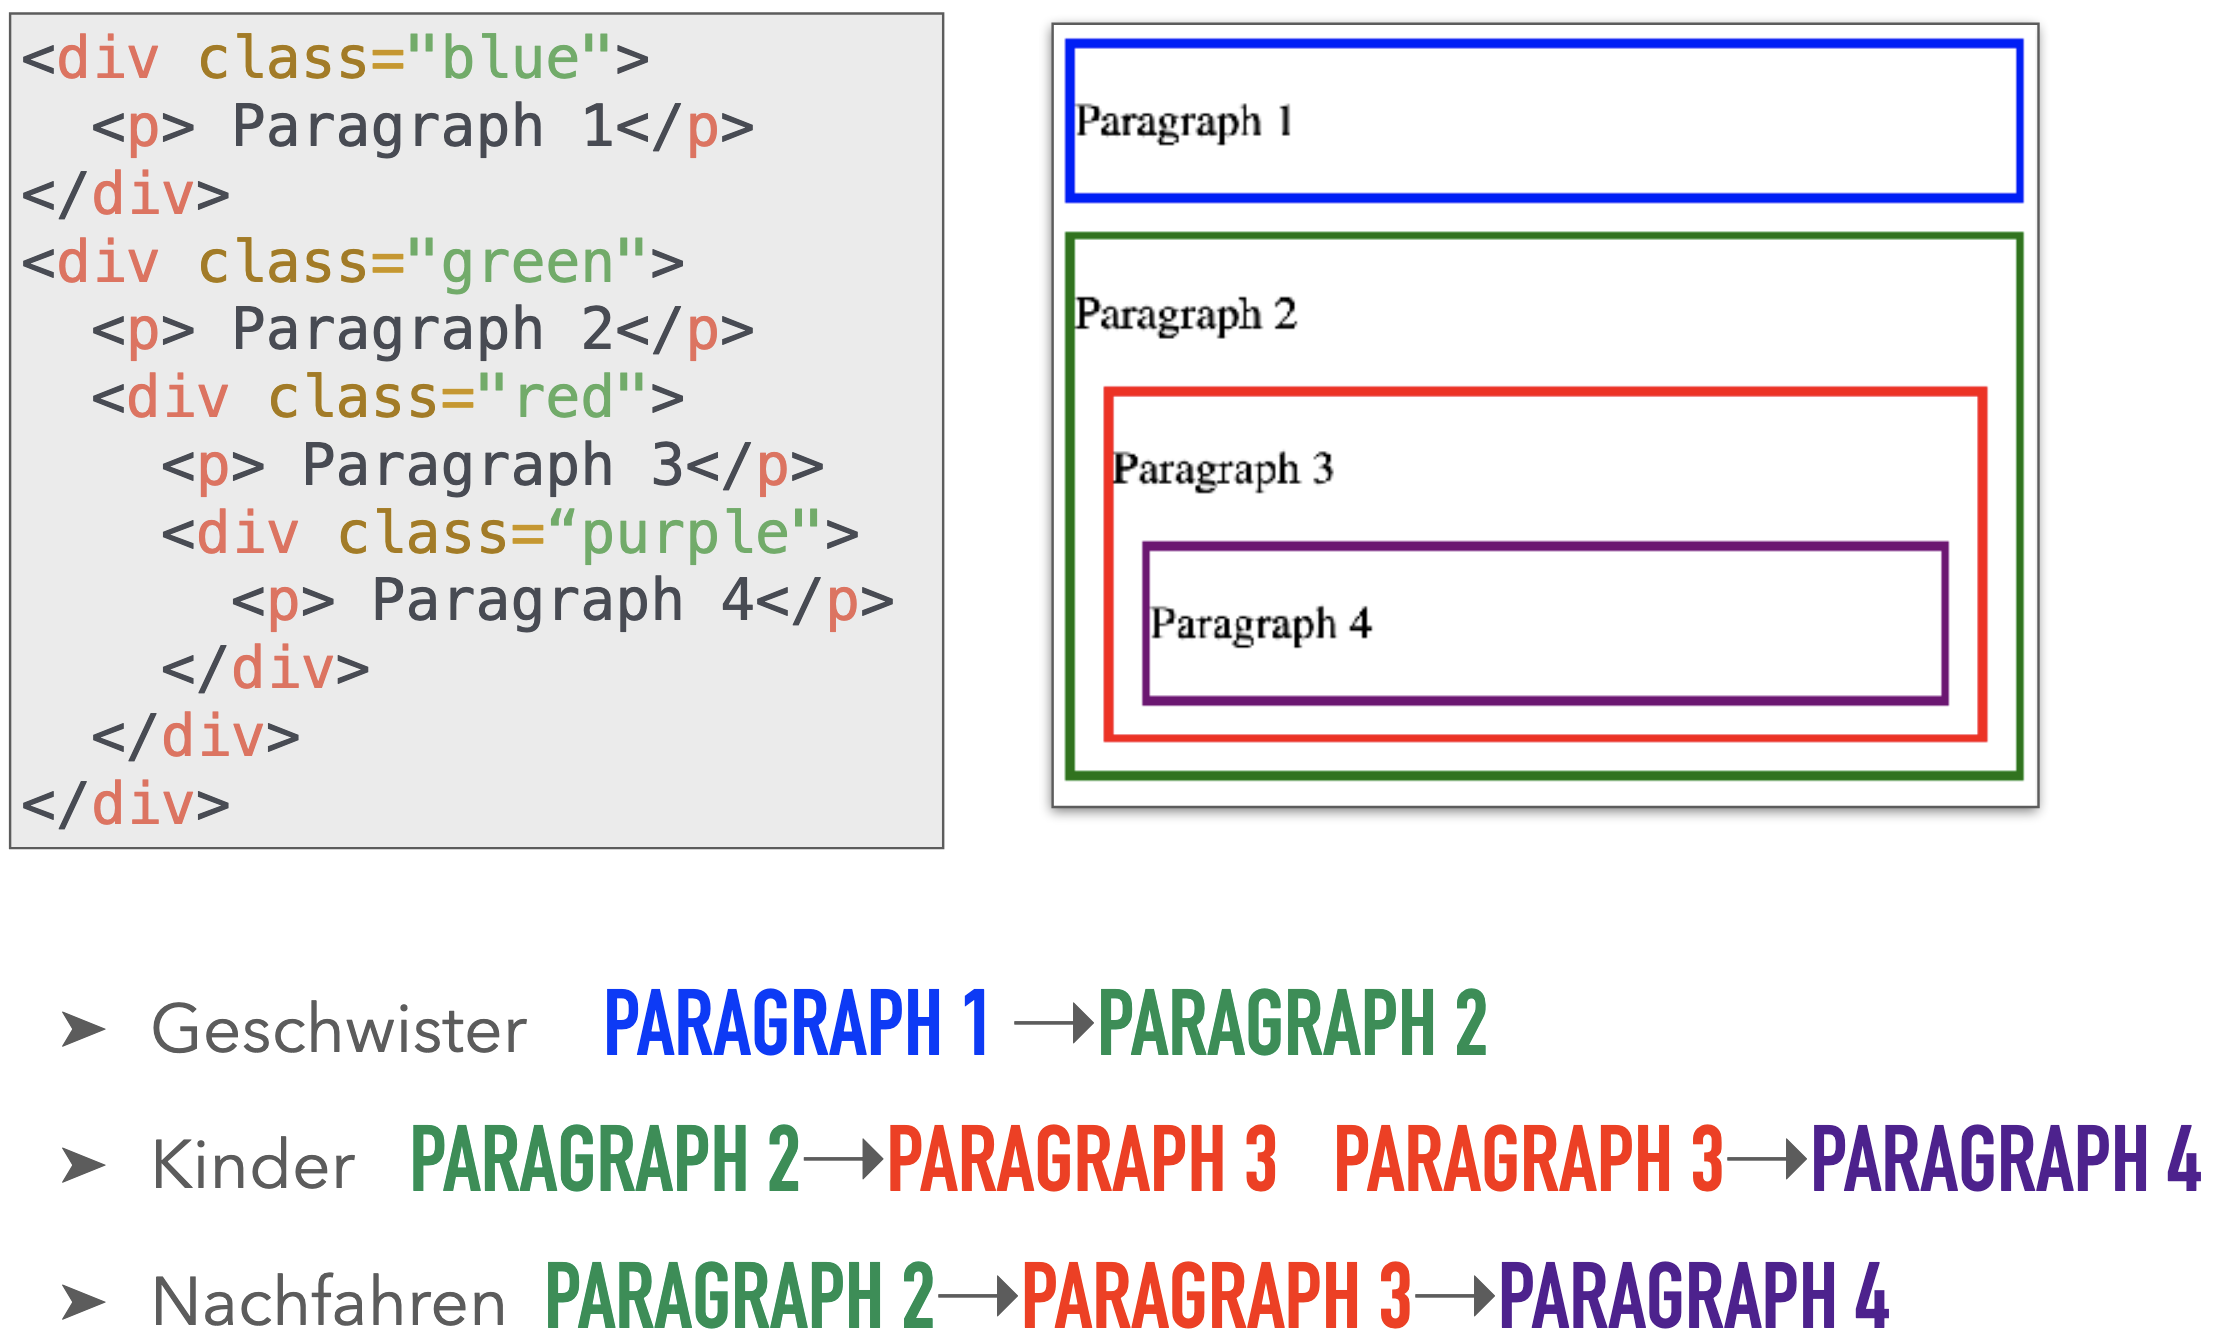
\includegraphics[scale=0.2]{Bilder/relations.png}
	\caption{Kinder, Nachbarn und Geschwister stehen in spezieller Relation}
	\end{wrapfigure}
	Hierbei muss man zuvor jedoch erst definieren, was ein Nachfahre, Kinder, Geschwister und Nachbarn sind.
	\begin{itemize}
		\item{Wenn ein Element von einem anderen Element umschlossen wird (Wenn also zum Beispiel ein Paragraph innerhalb eines divs stehen), dann ist jedes dieser Elemente ein Nachfahre.}
		\item{Ein Kind ist der Nachfahre welcher \textit{direkt} nach dem Element folgt.}
		\item{Wenn ein Element auf der selben Ebene als ein anderes Element innerhalb des selben Elements liegt, sind diese Geschwister.}
		\item{Ein Nachbar ist das Geschwisterelement, welches direkt \textit{direkt} nach dem Element folgt.}
	\end{itemize}
	\subsubsection{Cascading Order}
	Das Cascading in CSS stammt aus der Rangordnung aus welcher Elemente verändert werden. Es wurden bereits die verschiedenen Wege, wie man den Style eines Dokuments verändern kann, welche hier erneut relevant werden.
	\begin{enumerate}
		\item{Inline}
		\item{\texttt{<style>} Element im Header}
		\item{Externes CSS Stylesheet}
		\item{Standardeinstellung des Browsers}
	\end{enumerate}
	So hat ein Inlinestyle die höchste Priorität und der Browser die niedrigste. Wenn also das gleiche Attribut des gleichen Elements sowohl Inline als auch im externen Stylesheet verändert wird, wird der Style des Inline-CSS verwendet, da dieser eine höhere Priorität hat.
	\subsubsection{Specificity}
	Ein weiterer Aspekt des Cascading ist die Spezifizität von Elementen. Während zuvor dessen Quelle relevant war, ist nun wichtig, welches Attribut des Elements angesprochen wird.
	\begin{enumerate}
		\item{Style Attribut}
		\item{ID Attribut}
		\item{Class Attribut}
		\item{Element Attribut}
	\end{enumerate}
	Diese sind wiederum von der höchsten zur niedrigsten Spezifizität sortiert. Wenn also das gleiche Attribut des gleichen Elements mittels Inline Style und dem Element Selector verändert wird, hat der Inline Style eine höhere Priorität und wird anhand dessen gestyled.
	\subsubsection{Kommentare}
	Kommentare werden in CSS gleich wie in Java mit einem Slash und einem Stern eingeleitet und wiederum mit einem Stern und einem Slash beendet: \texttt{/* This is a CSS Comment */}
	\subsection{Text}
	Man kann in CSS auch spezifisch Text ansprechen. Die grundlegendste Veränderung ist dabei dessen Farbe zu ändern. CSS definiert dabei 140 Grundfarben welche mit einem Namen angesprochen werden können, diese sehen jedoch meist nicht allzu schön aus. Um diesen genauer zu verändern kann man diese auf drei Wege ansprechen:
	\begin{itemize}
		\item{RGB}
		\begin{itemize}
			\item{Besteht aus drei Werten zwischen 0 und 255 und gibt die Rot-, Grün- und Blauwerte an.}
			\item{Um eine Farbe in RGB anzugeben, muss man rgb vor die Klammer schreiben: \texttt{rgb(0, 255, 0)}}
		\end{itemize}
		\item{RGBA}
		\begin{itemize}
			\item{Funktioniert gleich wie RGB, hat jedoch zusätzlich den Alpha Channel, welcher die Deckkraft der Farbe angibt (Auch zwischen 0 und 255)}
			\item{Um eine Farbe in RGBA anzugeben, muss man rgb vor die Klammer schreiben: \texttt{rgba(0, 255, 0, 255)}}
		\end{itemize}
		\item{Hexadezimal}
		\begin{itemize}
			\item{Funktioniert gleich wie RGB, die Zahlen werden jedoch in Hexadezimalzahlen angegeben.}
			\item{Um eine Farbe als Hex anzugeben, muss man # for die Zahlen schreiben: \texttt{#00ff00}}
		\end{itemize}
		Weitere Attribute von Text sind das \texttt{text-alignment} und das \texttt{text-decoration}:
		\begin{itemize}
			\item{\texttt{text-alignment}}
			\begin{itemize}
				\item{Gibt die Bündigkeit des Textes an:}
				\begin{itemize}
					\item{Dabei sollte man jedoch beachten, dass diese Bündigkeit nur innerhalb der Grenzen des Elements geschieht und \textit{nicht} die Anordnung des Elements verändert.}
					\item{\texttt{left -> Linksbündig}}
					\item{\texttt{right -> Rechtsbündig}}
					\item{\texttt{center -> Zentriert}}
					\item{\texttt{justified -> Blocksatz}}
				\end{itemize}
			\end{itemize}
			\item{\texttt{text-decoration}}
			\begin{itemize}
				\item{Fügt dem Text weitere Elemente hinzu:}
				\begin{itemize}
					\item{\texttt{underline -> Unterstreicht den Text}
					\item{\texttt{line-through -> Unterstreicht den Text}}}
				\end{itemize}
			\end{itemize}
		\end{itemize}
		\subsubsection{Schriftart}
		Man kann auch die Schriftart des Textes ändern. Dabei bietet CSS die Möglichkeit eines Fallbacks an, welcher relevant wird, wenn der

	\end{itemize}
	\newpage
	\begin{tabular}{| l | l | l |}
		\toprule
		Name &  & & & \\ \midrule
		
		\bottomrule
	\end{tabular}
	\subsection{Text}





















  
\end{document}